\chapter{Results, Discussion, and Perspectives}
\label{ch:results}

This chapter reports the measurements obtained, assesses what they do and
do not establish, and sets out perspectives for continuing the work. All
figures quoted are read directly from the serialised evaluation artefacts
in \file{checkpoints/} --- principally \file{eval_metrics.json},
\file{heldout/heldout_validation.json} and the two
\file{guidance_diagnostics_*.json} files --- rather than transcribed
from run logs.

\section{Evaluation Protocol}

Following Singla~\emph{et al.}~\cite{singla2022}, the evaluation set is
split by classifier confidence into a negative group
$X_n = \{x : f(x) < 0.2\}$ and a positive group
$X_p = \{x : f(x) > 0.8\}$, with up to $n_{\text{eval}} = 200$ images
each. The \ntop{} policy generates counterfactuals from $X_n$ toward
$c=1$; the \pton{} policy generates from $X_p$ toward $c=0$. Both use the
policy's deterministic mean action, for reproducibility.

The metric suite comprises Counterfactual Validity (CV), Fr\'echet
Inception Distance (FID)~\cite{heusel2017fid} computed in
TorchXRayVision DenseNet feature space rather than ImageNet Inception
space, a model-free Identity Preservation (IP) score, and two clinical
proxy metrics --- Cardio-Thoracic Ratio (CTR) and a costophrenic-recess
score (SCP) --- each tested with a paired $t$-test on the within-image
delta.

\subsection{Identity Preservation as a Substitute for FOP}

The reference protocol's Foreign-Object Preservation metric requires a
Fast R-CNN device detector trained on private, manually annotated data.
It is not reproducible offline, and no TorchXRayVision weight set exposes
a usable ``Support Devices'' head. FOP is accordingly reported as
\textbf{unavailable} --- it is serialised as \texttt{null} in
\file{eval_metrics.json}, not silently omitted --- and substituted by a
model-free IP score measuring the same underlying property:

\begin{itemize}[leftmargin=*]
  \item \textbf{MS-SSIM}~\cite{wang2003msssim}: multi-scale structural
        similarity between $x$ and $x_c$, capturing global anatomical
        identity.
  \item \textbf{HF-corr}: Pearson correlation between high-pass-filtered
        versions of $x$ and $x_c$. Thin, high-contrast structures ---
        tubes, leads, pacemakers --- are exactly the spatial-frequency
        content a Gaussian high-pass isolates, making this a direct proxy
        for whether such hardware survives editing.
\end{itemize}

\section{Obtained Results}

\subsection{Primary Metric Suite}

\begin{table}[h]
\centering
\caption[Primary evaluation metric suite]{Evaluation results from \file{checkpoints/eval_metrics.json},
$n_{\text{eval}} \le 200$ per group. FID is computed between each real
group and its own counterfactual set.}
\label{tab:results}
\begin{tabular}{@{}llrr@{}}
\toprule
\textbf{Metric} & \textbf{Definition} & \textbf{\ntop{}} & \textbf{\pton{}} \\
\midrule
CV        & fraction valid ($\tau = 0.8$)      & 0.995 & 0.955 \\
          & \textit{mean}                       & \multicolumn{2}{c}{0.975} \\
FID       & XRV-DenseNet features, lower better & 103.83 & 59.73 \\
IP        & MS-SSIM                             & 0.849 & 0.796 \\
IP        & HF-corr                             & 0.938 & 0.798 \\
FOP       & not computable offline              & --- & --- \\
\bottomrule
\end{tabular}
\end{table}

Counterfactual Validity is high in both directions. Section~\ref{sec:heldout}
explains why this number, taken alone, is not evidence of success.

Identity preservation is respectable and consistently better for the
\ntop{} direction (MS-SSIM $0.849$, HF-corr $0.938$) than for \pton{}
($0.796$, $0.798$), indicating that fine high-frequency structure ---
the hardware the HF-corr proxy is designed to track --- survives editing
substantially better when adding a pattern than when removing one.

The FID values are high in absolute terms. Two factors compound here.
The estimates use $N \approx 200$ samples against a 1024-dimensional
feature space, far below the sample count FID nominally requires, so
their variance is large. Beyond that, they indicate a genuine
distributional gap between generated and real radiographs that the
current training budget did not close. These should be read as
directionally informative --- \pton{} is clearly the more realistic
direction --- rather than as tightly bounded estimates.

\subsection{Clinical Proxy Metrics}

\begin{table}[h]
\centering
\caption[Clinical proxy metrics]{Clinical proxy metrics: group means $\pm$ standard deviation and
paired $t$-tests on the within-image real$\rightarrow$counterfactual delta.
Significance at $\alpha = 0.05$ marked with $^{\ast}$.}
\label{tab:clinical}
\begin{tabular}{@{}lccr@{}}
\toprule
& \textbf{Real group} & \textbf{Counterfactual} & \textbf{$\Delta$ ($t$, $p$)} \\
\midrule
\multicolumn{4}{@{}l}{\textit{\ntop{} direction ($X_n \rightarrow X_c^{n\to p}$)}}\\
CTR & $0.424 \pm 0.055$ & $0.417 \pm 0.078$ & $+0.0070$ \ ($t=1.09$, $p=0.276$) \\
SCP & $0.4794 \pm 0.0008$ & $0.4795 \pm 0.0009$ & $-0.00014$ \ ($t=-2.89$, $p=0.0042^{\ast}$) \\
\midrule
\multicolumn{4}{@{}l}{\textit{\pton{} direction ($X_p \rightarrow X_c^{p\to n}$)}}\\
CTR & $0.452 \pm 0.101$ & $0.452 \pm 0.131$ & $+0.0251$ \ ($t=2.22$, $p=0.028^{\ast}$) \\
SCP & $0.4791 \pm 0.0010$ & $0.4792 \pm 0.0011$ & $-0.00012$ \ ($t=-1.52$, $p=0.129$) \\
\bottomrule
\end{tabular}
\end{table}

The picture here is mixed and should not be overstated. Only two of the
four tests reach significance, and they are not the same two: CTR shifts
significantly in the \pton{} direction but not in \ntop{}, while SCP does
the reverse.

The CTR result is arguably the more interpretable of the two, and it is
interpretable as a \emph{success of the spatial constraint}. The
cardio-thoracic ratio is driven by the cardiac silhouette, which lies
largely outside the pure lung mask that gates editing. A system whose
background lock is working should therefore leave CTR nearly unchanged
--- which is what the small absolute magnitudes ($0.007$ and $0.025$
against group means near $0.43$) show. The SCP deltas are smaller still,
around $10^{-4}$ on a metric with a standard deviation near $10^{-3}$;
their statistical significance reflects the paired design and $n \approx 200$
rather than any clinically meaningful shift.

The honest summary is that the clinical proxy metrics are not currently
discriminative enough to support conclusions about clinical realism.
Section~\ref{sec:limitations} explains why the SCP proxy in particular
should be treated as a weak instrument.

\subsection{Qualitative Counterfactuals}

\begin{figure}[h]
  \centering
  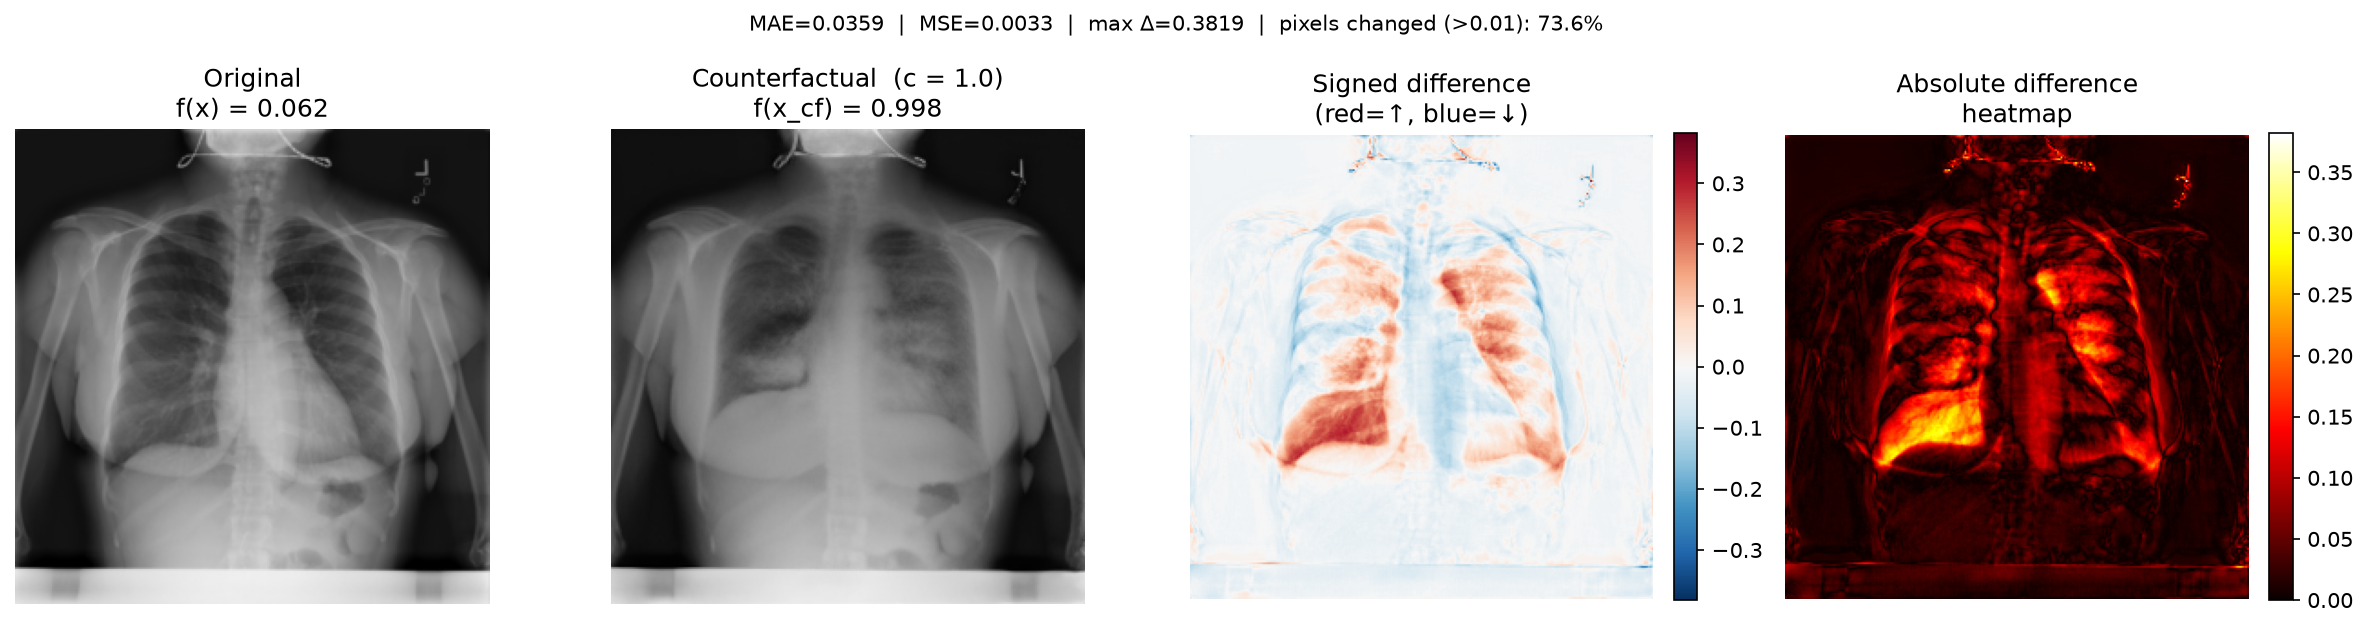
\includegraphics[width=\textwidth]{counterfactual_diff_n_to_p.png}
  \caption[Counterfactual: normal to pneumonia]{\textbf{Normal $\rightarrow$ pneumonia.} Left to right:
  original, counterfactual targeting $c=1$, signed pixel difference, and
  absolute-difference heatmap, produced by \file{src/diff_viz.py}. The
  classifier score crosses the decision boundary by a wide margin.}
  \label{fig:n2p}
\end{figure}

\begin{figure}[h]
  \centering
  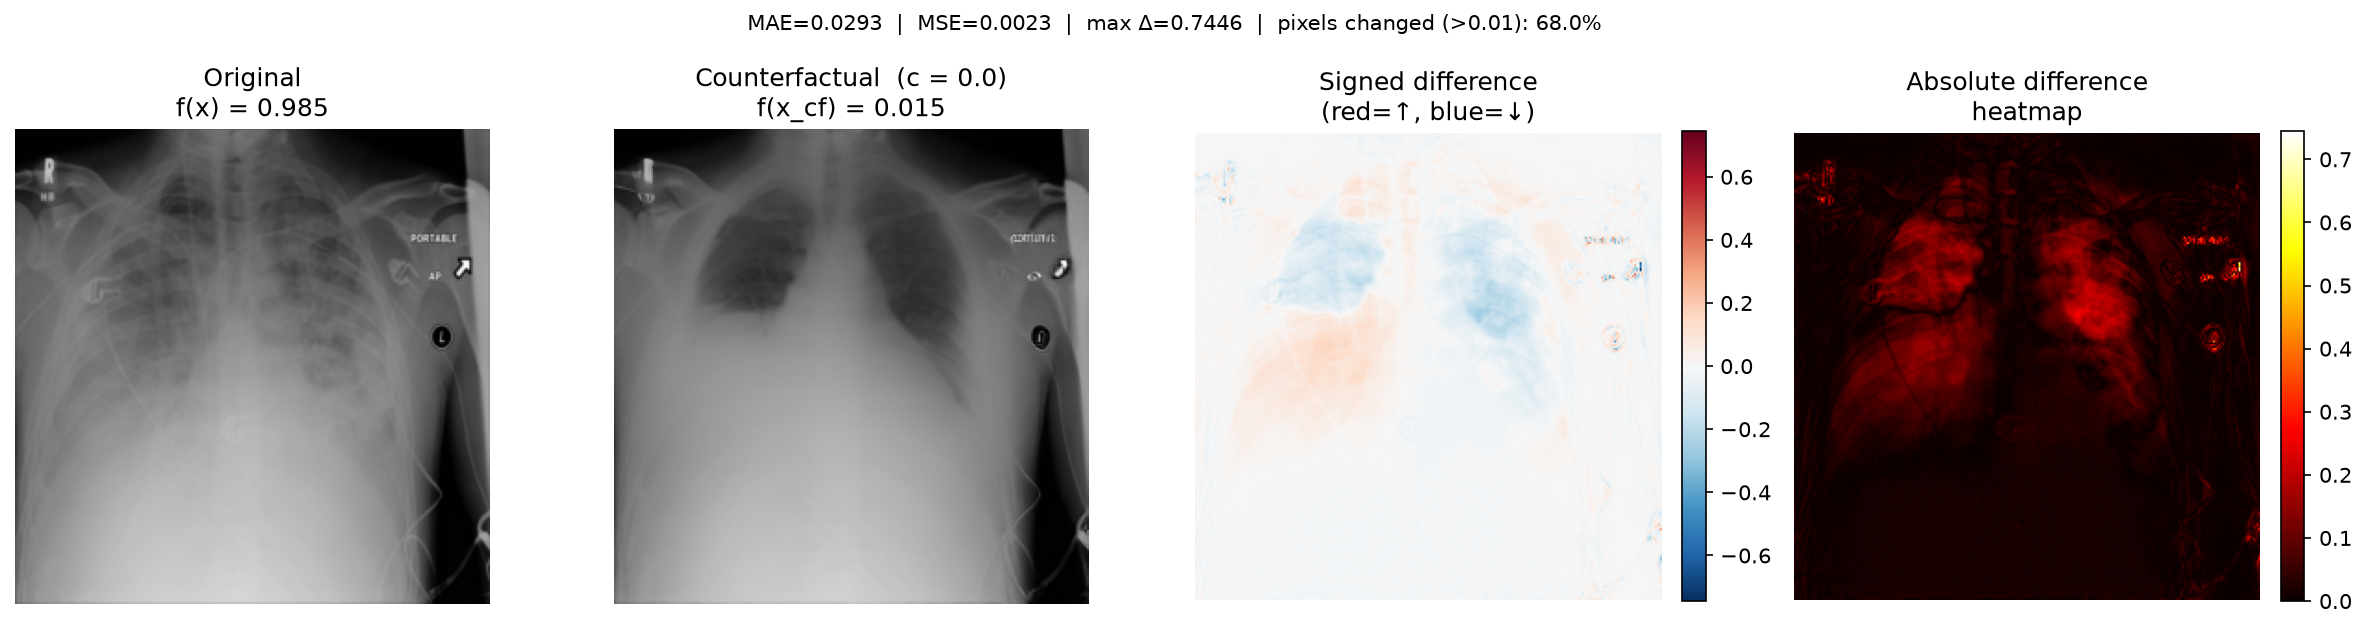
\includegraphics[width=\textwidth]{counterfactual_diff_p_to_n.png}
  \caption[Counterfactual: pneumonia to normal]{\textbf{Pneumonia $\rightarrow$ normal.} Same four-panel
  layout. Change is distributed over both lung fields, consistent with
  opacity removal, and at a lower overall magnitude than the \ntop{} case
  --- MAE $0.029$ versus $0.042$, as measured over 200 images per
  direction in \file{heldout_validation.json}.}
  \label{fig:p2n}
\end{figure}

Gross anatomical layout outside the lung field is visibly retained in
both directions, which is the qualitative signature of the background
lock holding as designed.

\subsection{Training Diagnostics}

\begin{figure}[h]
  \centering
  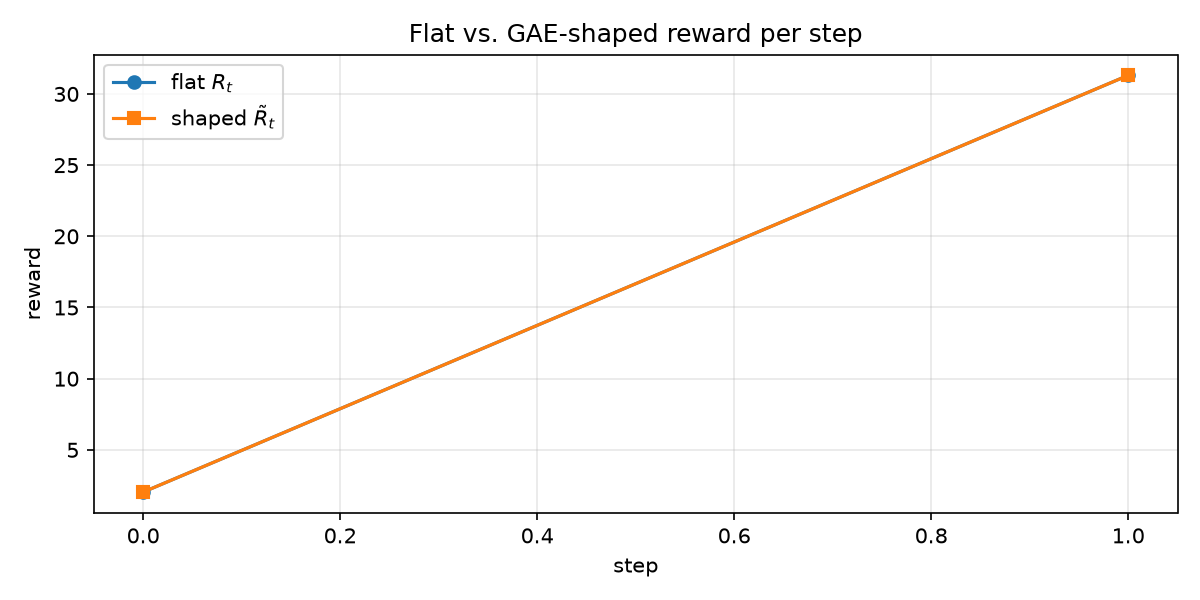
\includegraphics[width=0.72\textwidth]{reward_trace.png}
  \caption[PPO reward trace diagnostic]{Flat per-step reward $R_t$ against the GAE-shaped reward
  $\tilde R_t$ over a short post-training rollout
  (\file{factory/evaluate.py}, \texttt{plot\_reward\_trace}). The trace is
  short because this rollout reaches validity almost immediately, and the
  two curves are near-coincident --- a direct consequence of PPO's
  per-update advantage normalisation absorbing a uniform shaping term.
  This is a training-health diagnostic, not a convergence curve.}
  \label{fig:reward}
\end{figure}

The guidance diagnostics serialised alongside each policy checkpoint show
that the two directions converged to visibly different control
strategies. The \ntop{} policy settles at a guidance bias of $1.298$ ---
essentially the top of its $[0.70, 1.30]$ range --- meaning it maximally
favours classifier guidance over preservation, and suppresses
preservation to a factor of $0.771$. The \pton{} policy does the
opposite, settling at $0.701$, the bottom of the range, which
\emph{amplifies} preservation by $1.428\times$. Average reward differs
accordingly: $21.41$ for \ntop{} against $14.87$ for \pton{}.

Both policies pin their guidance bias to opposite ends of the available
range, with standard deviations below $0.006$. This near-deterministic
saturation indicates the action bound, not the policy, is the binding
constraint on this dimension --- a concrete signal that the range itself
should be widened in future work.

\section{The Held-Out Validation Result}
\label{sec:heldout}

The central experimental finding of this internship is negative, and it
concerns the interpretation of Table~\ref{tab:results}.

Counterfactual Validity there is computed with the same classifier that
generated the guidance gradient. To test whether the edits carry disease
signal rather than a perturbation tailored to that one model, job
\textbf{17649721} re-scored 200 counterfactuals per direction with two
TorchXRayVision DenseNet-121 classifiers that had never participated in
guidance.

\begin{table}[h]
\centering
\caption[Held-out validation results]{Held-out validation (\file{checkpoints/heldout/heldout_validation.json}),
$n=200$ per direction, $\tau=0.8$. Guidance classifier at generation time:
\texttt{densenet121-res224-rsna} alone. Strict CV is the fraction of
counterfactuals each validator independently judges valid.}
\label{tab:heldout}
\begin{tabular}{@{}llrrr@{}}
\toprule
\textbf{Classifier} & \textbf{Role} & \textbf{CV \ntop{}} & \textbf{CV \pton{}} & \textbf{Agreement} \\
\midrule
\texttt{-rsna}  & guidance (circular) & 0.995 & 0.885 & --- \\
\texttt{-chex}  & held out            & 0.080 & 0.000 & 0.707 \\
\texttt{-nih}   & held out            & 0.000 & 0.000 & 0.697 \\
\bottomrule
\end{tabular}
\end{table}

The gap is stark. Counterfactuals that the guidance classifier accepts
99.5\% of the time are accepted by an independent classifier at most 8\%
of the time, and in three of the four held-out cells, never. Transfer
ratios --- the fraction of the guidance model's score shift that the
validators reproduce --- are $0.205$ and $0.590$ for \ntop{} and only
$0.132$ and $0.143$ for \pton{}.

The agreement control is what makes this conclusive. On the
\emph{original}, unedited images the validators agree with the guidance
classifier around 70\% of the time ($0.697$ and $0.707$), confirming they
share a working notion of the task. They are not failing to recognise
pneumonia in general; they are failing to recognise it in these specific
generated images.

The conclusion is direct: \textbf{the \pton{} direction in particular was
not removing disease, it was fooling $f(\cdot)$.} The edits were largely
adversarial perturbations against the guidance classifier rather than
semantic changes to depicted pathology.

The edit-concentration figures recorded in the same artefact corroborate
this. Concentration --- the share of total absolute change carried by the
top 5\% of pixels --- was $0.282$ (\ntop{}) and $0.297$ (\pton{}) against
a uniform baseline of $0.05$, with 66\% and 62\% of all pixels changed
and MAE of $0.042$ and $0.029$. A focal consolidation should concentrate
well above $0.5$. These edits have a concentrated core but carry most of
their mass in a diffuse, low-amplitude tail spread over the majority of
the image --- the visual signature of an adversarial perturbation rather
than a lesion.

This result motivated the three countermeasures described in
Chapter~\ref{ch:tasks}: ensemble guidance, the Grad-CAM action-space
constraint, and the annealed sparsity reward.

\subsection{Status of the Countermeasures}
\label{sec:status}

The countermeasures are \textbf{implemented and enabled} in
\file{config.py}, and a training run under the new configuration was in
progress at the close of the internship: the most recent log
(job \textbf{17653310}) shows the ensemble classifier loading correctly
with both members, the Grad-CAM mask active, and the sparsity ramp
resolved over updates $[20, 60)$ of 100.

\textbf{A re-run of the held-out validation against the new configuration
was not completed within the internship period.} Whether ensemble
guidance, spatial constraint and sparsity pressure actually close the
transfer gap in Table~\ref{tab:heldout} is therefore an open question,
not a demonstrated result. It is the first item of future work in
Section~\ref{sec:future}.

The one measurement available from the new configuration is a caution
rather than a result: the pipeline log notes that Grad-CAM is degenerate
for one of the two ensemble members, so the constraint mask is
effectively being computed from a single member. The ensemble-aware CAM
path handles this by averaging over the remaining members instead of
failing, but it means the spatial constraint is currently weaker than the
design intends.

\section{Strengths and Limitations}

\subsection{Strengths}

\begin{itemize}[leftmargin=*]
  \item \textbf{A genuine spatial guarantee.} The background lock is a
        structural constraint rather than a penalty term. Content outside
        the lung field cannot be repainted regardless of the guidance
        gradient's behaviour, and the small CTR deltas in
        Table~\ref{tab:clinical} are consistent with it holding.
  \item \textbf{Parameter-efficient adaptation.} Domain adaptation of an
        866M-parameter generator was achieved by training 0.78\% of its
        parameters, which is what made the project feasible within a
        single-GPU budget.
  \item \textbf{Sampling control without weight modification.} The PPO
        agent never touches the diffusion weights, keeping the action
        space interpretable at 9 bounded dimensions and the learned
        policy reusable across arbitrary query images.
  \item \textbf{Falsifiable evaluation.} The project's most valuable
        output is a control that exposed its own primary metric as
        circular. The held-out validation apparatus, its agreement
        control, and the disjointness rule between guidance and validator
        sets are reusable well beyond this system.
\end{itemize}

\subsection{Limitations}
\label{sec:limitations}

\begin{itemize}[leftmargin=*]
  \item \textbf{Transfer to independent classifiers is unresolved.} This
        is the principal limitation. As of the end of the internship the
        counterfactuals demonstrably did not transfer
        (Section~\ref{sec:heldout}), and the countermeasures are
        implemented but unvalidated (Section~\ref{sec:status}).
  \item \textbf{FOP is not computable.} The reference metric requires an
        unavailable detector, and the IP substitute measures a related
        but not identical property.
  \item \textbf{SCP is a weak proxy.} It is derived from a COCO-pretrained
        YOLOv8 feature norm rather than a dedicated costophrenic-recess
        detector. Its near-zero deltas in Table~\ref{tab:clinical} should
        not be read as clinical measurements.
  \item \textbf{FID estimates are imprecise and high.} $N \approx 200$
        against a 1024-dimensional feature space gives wide error bars,
        and the absolute values indicate a real realism gap.
  \item \textbf{Compute-constrained training scale.} The episode and
        epoch budgets are documented in \file{config.py} as conservative
        placeholders sized for the available walltime, not values
        established by ablation.
  \item \textbf{Two independently trained policies.} A single
        target-conditioned policy would let the harder direction share
        representation capacity with the easier one, but requires an
        environment refactor not undertaken here.
  \item \textbf{No baseline comparison was performed.} No GAN-based
        counterfactual baseline was implemented or evaluated within this
        internship, so the system's performance is not positioned against
        prior work. This is stated explicitly because it is a real gap in
        the evaluation, not an oversight in reporting.
  \item \textbf{Single dataset, single pathology.} All results concern
        binary pneumonia classification on RSNA. Nothing here establishes
        generalisation to other pathologies, other corpora, or other
        acquisition protocols.
\end{itemize}

\section{Perspectives and Future Work}
\label{sec:future}

\begin{itemize}[leftmargin=*]
  \item \textbf{Complete the validation loop (highest priority). ---
        \emph{Resolved in Chapter~\ref{ch:closing}.}} Chapter~\ref{ch:integrity}
        showed ensemble guidance helps on no-policy arms; Chapter~\ref{ch:closing}
        retrains both directional policies from scratch under it and
        re-scores them against \texttt{\{nih, pc, mimic\_ch\}} (the leak-free
        validator set, since \texttt{chex} is now a guidance member). Mean
        transfer improves on both directions ($0.230\to0.282$ \ntop{},
        $0.146\to0.293$ \pton{}), but \texttt{nih}'s \ntop{} ratio does not
        ($0.080\to0.046$) --- a partial, not complete, closure of the gap.
  \item \textbf{Resolve the trained-vs-random paired significance test. ---
        \emph{Resolved in Chapter~\ref{ch:closing}.}}
        Table~\ref{tab:lhr_arms} in Chapter~\ref{ch:integrity} shows trained
        editing toward a higher LHR lift than random ($2.293$ vs.\ $2.204$)
        at the group level; \S\ref{sec:closing_significance} runs
        \file{paired\_arm\_test.py}'s per-image paired test on the same 183
        images and finds the gap survives ($p=0.012$) at a small effect size
        ($d=0.19$).
  \item \textbf{Run the ablation arms.} The \texttt{SMOKE\_ARM}
        infrastructure (\texttt{baseline} / \texttt{mask} / \texttt{all})
        is already in place to attribute any improvement to the
        individual mechanisms rather than to their combination.
  \item \textbf{Diagnose why the Grad-CAM constraint hurts lesion
        targeting.} Chapter~\ref{ch:integrity} found the Grad-CAM mask
        (ARM~2) measurably \emph{lowers} LHR lift relative to baseline,
        both alone and combined with ensemble guidance --- the opposite of
        its intended effect. With Grad-CAM degenerate for one ensemble
        member, the spatial constraint may be operating on an unreliable
        mask; diagnosing that is now a more concrete, more urgent version
        of this item than when it was first identified.
  \item \textbf{Widen the guidance-bias action range.} Both policies
        saturate at opposite ends of $[0.70, 1.30]$ with near-zero
        variance, indicating the bound rather than the policy is binding.
  \item \textbf{Increase evaluation sample size.} The single most direct
        lever on FID precision.
  \item \textbf{Implement a baseline comparison.} A GAN-based
        counterfactual generator evaluated under an identical protocol
        would place these results in context.
  \item \textbf{Unify the two policies.} A single target-conditioned
        policy with randomised per-episode target would be
        architecturally cleaner and would let the harder \ntop{}
        direction borrow capacity from the easier one.
  \item \textbf{Broaden scope.} Extending beyond binary pneumonia to
        multi-pathology counterfactuals, and to a second corpus, would
        test whether any of this generalises.
\end{itemize}

\section{Conclusion}

This chapter has reported the system's measured performance and
subjected it to an independent control that substantially qualifies it.
High counterfactual validity against the guidance classifier proved not
to survive contact with classifiers that never guided it. The
countermeasures this motivated are built and running, but their
effectiveness is not yet established. The following general conclusion
reflects on what the internship produced and what it taught.
